\begin{intro}
\label{intro}

En la naturaleza, es posible encontrar de forma ubicua, estructuras alargadas (filamentos), las que conforman redes entre sí. La conformación de estas estructuras complejas y din\'amicas se puede observar en ejemplos particulares como en una red de prote\'inas de una c\'elula eucariota, as\'i como en bacterias, ya que a pesar que pertenecer a distintas familias, ambas tienen estructuras formada por filamentos. 
Caracter\'isticas f\'isicas de estas redes generan propiedades tales como la presencia o ausencia de ciclos, o la posibilidad de dividir o no cada filamento. Por su parte, el análisis de filamentos que conforman la red, puede indicar el estado de \'esta, respecto a su ambiente o de su interior, as\'i como develar informaci\'on relevante sobre la relaci\'on entre la estructura biol\'ogica y funciones fisiol\'ogicas.  
%movimiento interno, reparación de tejido,
% estructuras dinamicas y complejas que juegan varios roles
% A modo de ejemplo, una red de proteinas de una c\'elula eucariota contiene tres tipos de filamentos en la constituci\'on de su citoesqueleto: microfilamentos, microt\'ubulos y filamentos intermedios. Sin embargo, una estructura de citoesqueleto también existe en una bacteria.
  
\vspace{.5cm}
Los m\'etodos actuales para analizar las redes mencionadas se basan en el procesamiento directo de im\'agenes obtenidas a partir de microscop\'ia (Figura \ref{Fig1a}), pasando por etapas de segmentaci\'on (Figura \ref{Fig1b}), para luego utilizar diversas t\'ecnicas como esqueletonizaci\'on (Figura \ref{Fig1c}), la transformada de Rad\'on o {\it template matching}. Esto permite identificar el grafo que representa a la red (Figura \ref{Fig1d}) o sirve de base para el uso de heur\'isticas que permiten identificar los filamentos de forma individual.
 %como tambi\'en pueden utilizarse una esqueletonizaci\'on de la misma (Figura \ref{Fig1c}), o la construcci\'on de un grafo (Figura \ref{Fig1d}), entre otras.
 % En todos estos casos, el objetivo radica en
La individualizaci\'on de filamentos permite cuantificar las propiedades de la red tales como n\'umero de filamentos, largo de estos, volumen, o curvatura. Estos m\'etodos, basados en la observaci\'on mediante microscop\'ia \'optica tienen como cota m\'axima de resoluci\'on el l\'imite de difracci\'on, $\lambda/2$. Donde $\lambda$ es la longitud de onda de la luz utilizada (o color). Este l\'imite establece que 2 objetos cuya distancia sea inferior a $\lambda/2$ no pueden ser diferenciados, conllevando a que dos partes del grafo cercanos puedan ser observadas como una, dificultando su estudio. Lo anterior es relevante para asociar las propiedades de la red a los v\'ertices del grafo extra\'ido, dando pie a la caracterizaci\'on del mismo (Figura \ref{Fig2a}).
 % vertices del grafo extraido, que representan a un filamento de forma individual, 
 
 \begin{figure*}[h!]
    \centering
    \label{fig:flujo-expected}
    \begin{subfigure}[t]{0.5\textwidth}
        \centering
        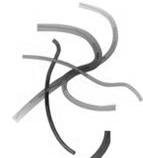
\includegraphics[height=1.5in]{imagenes/define-weighted-4.png}
        \caption{Representaci\'on simplificada de una red con cruces y sobreposici\'on de filamentos en una imagen de microscop\'ia.}
        \label{Fig1a}
    \end{subfigure}%
    ~ 
    \begin{subfigure}[t]{0.5\textwidth}
        \centering
        
\includegraphics[height=1.5in]{imagenes/define-weighted-4-bw-invert.png}
        \caption{Preprocesamiento de la imagen mediante segmentaci\'on para la extracci\'on de la red.}
        \label{Fig1b}
    \end{subfigure}
    %\caption{Caption place holder}
%\end{figure*}
\vskip\baselineskip
%\begin{figure*}[t!]
%    \centering
    \begin{subfigure}[t]{0.5\textwidth}
        \centering
        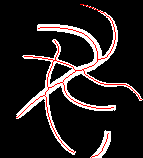
\includegraphics[height=1.5in]{imagenes/skel_in_segment.png}
	    \caption{Esqueletonizaci\'on representativa de la red sobre la imagen de \ref{Fig1b}.}
        \label{Fig1c}
    \end{subfigure}%
    ~ 
    \begin{subfigure}[t]{0.5\textwidth}
        \centering
        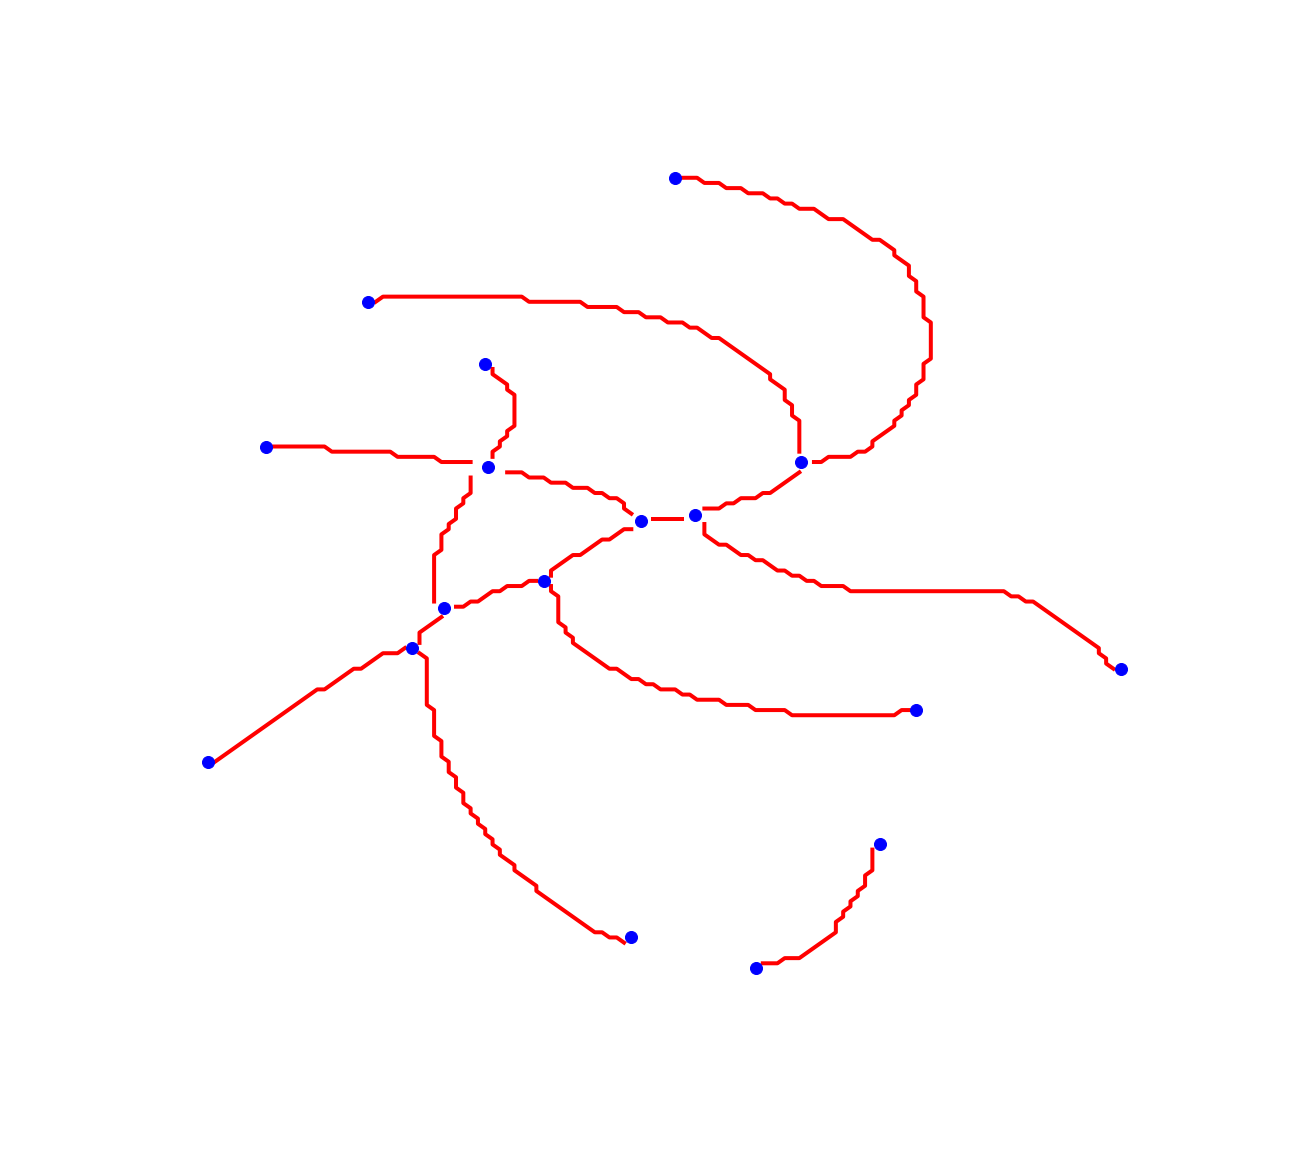
\includegraphics[height=1.5in]{imagenes/graph_of_skel_no_axis.png}
        \caption{Grafo que representa la esqueletonizaci\'on de la red.}
        \label{Fig1d}
    \end{subfigure}
%    \vskip\baselineskip
    \caption{Procedimiento para obtener un grafo que representa la red, a partir del procesamiento de una imagen de microscop\'ia, utilizando segmentaci\'on y esqueletonizaci\'on. Fuente: \cite{breuer2015define}}
\end{figure*}

Existen investigaciones en la literatura que apuntan a las distintas etapas de este problema, las que tienen en com\'un el uso de t\'ecnicas del \'area de procesamiento de im\'agenes para el tratamiento inicial de la imagen de microscop\'ia. La individualizaci\'on de filamentos puede ser categorizado en: basado en procesamiento de im\'agenes o como un problema de optimizaci\'on. 

\medskip
En la primera categor\'ia se encuentran enfoques asociados al an\'alisis de la reconstrucci\'on de filamentos en base a sus segmentos \cite{zhang2017extracting}, o relacionados a la extracci\'on de cada uno de los filamentos que conforman la red (\textit{Individual Fiber Segmentation}) a partir de una imagen \cite{doi:10.1021/ma502264c}\cite{boudaoud2014fibriltool}\cite{lichtenstein2003quantitative}\cite{alioscha2016robust}\cite{xu2015soax}. Para estos m\'etodos, se han indicado como cr\'iticas la dificultad para identificar correctamente un filamento de otro, en los casos de  superposici\'on, fragmentaci\'on, o variaciones de intensidad en la imagen.
% describir alguno de estos papers 

En la segunda categor\'ia, \cite{cerda2014geometrical} plantea la identificaci\'on de segmentos de filamentos como un problema de asignaci\'on, utilizando las medidas de distancia euclidiana y angular como restricciones, y el algoritmo h\'ungaro para su resoluci\'on. En la misma categor\'ia, \cite{breuer2015define} realiza la asociaci\'on de la red con un grafo no dirigido con pesos, en el que cada filamento es equivalente a un camino en el grafo. Esto permite que la b\'usqueda e individualizaci\'on de filamentos, con un segmento de filamento representado por una arista del grafo, sumado a las restricciones que plantea el autor, sea tratado como un problema de {\it Set Cover}. En el caso de los m\'etodos de la segunda categor\'ia, la mayor cr\'itica es su costo computacional alto, lo que limita en parte aquel enfoque. Se debe agregar que los par\'ametros utilizados por estas t\'ecnicas (\'angulos o  distancias m\'aximas entre filamentos) son complejas de obtener de los expertos directamente. Sin embargo, una de sus ventajas es que automatizan la recuperaci\'on de informaci\'on incluyendo una mayor cantidad de propiedades a cada arista. 

%representa un camino en este grafo, y los conjuntos de caminos 
\medskip
%Todos estos enfoques, cuya entrada principal de datos son las im\'agenes etiquetadas a trav\'es de marcadores fluorescentes, 
% basados en grafos

A modo de ejemplo, el programa \texttt{DeFine} desarrollado en \cite{breuer2015define} describe el problema de identificaci\'on de filamentos como un problema de b\'usqueda de caminos, es decir, como un problema del tipo {\it Path Cover}. Se define el peso de cada segmento/arista por un c\'alculo de {\it aspereza}, asociada al grosor o intensidad de la arista o un conjunto de estas.
%, o tambi\'en puede ser calculado respecto al \'angulo entre aristas.
Este problema particular es llamado {\it Filament Covering Problem} (FCP) y los autores demuestran que es NP-Hard, por lo que proponen un algoritmo de aproximaci\'on mediante \textit{Set Cover}, cuyo objetivo es que cada arista pertenezca al menos a un conjunto. La definici\'on de {\it Set Cover} es:

\begin{quote}
Dado un conjunto de elementos, denominado universo, y $n$ conjuntos cuya unión comprende el universo, el {\it Set Cover Problem} consiste en identificar el menor n\'umero de conjuntos cuya unión a\'un contiene todos los elementos del universo.
\end{quote}

La adaptaci\'on a lo definido por {\it FCP} es: 
\begin{quote}
Sea el universo $U$ conformado por las aristas del grafo, y un conjunto $S$, conformado por conjuntos de aristas, cada uno con costo $c_s$, $s \in S$:

Encontrar un subconjunto $S_{set} \subseteq S$ con costo m\'inimo (o promedio, dependiendo de la forma en que se calcula la aspereza) tal que cada elemento en $U$ este cubierto al menos una vez.
\end{quote}

Con la demostraci\'on de que FCP es NP-Hard, dado que la cantidad de caminos crece de forma exponencial respecto al n\'umero de nodos, los autores de \cite{breuer2015define} plantean la elecci\'on de un subconjunto de caminos, con los que pueden expresar el problema de {\it Set Cover} como algoritmo de aproximaci\'on lineal fraccional binario. El subconjunto de caminos puede obtenerse con la heur\'istica de recorrer el grafo por su anchura ({\it Breadth-First Search}), deteni\'endose al momento que el \'angulo de deflexi\'on entre aristas adyacentes supere 60\degree, o de caminos generados a partir de 100 \'arboles de expansi\'on m\'inima aleatoria ({\it RMST}), aportando cada uno de los 100 con $N(N-1)/2$ caminos no triviales y sin direcci\'on. El flujo de decisiones para generar el subconjunto de caminos puede observarse en la figura \ref{fig:define-set-cover}.

\begin{figure*}[h!]
    \centering
    \label{fig:flujo-expected}
    \begin{subfigure}[t]{\textwidth}
        \centering
        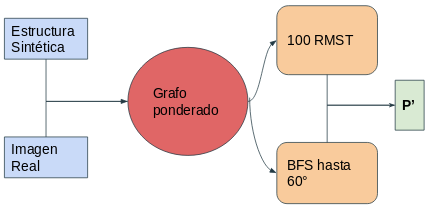
\includegraphics[scale=0.5]{imagenes/flujoDefine.png}
        \caption{Entrada de datos y elecci\'on de subconjunto de caminos {\bf P'} en DeFine.}
        \label{fig:define-set-cover}
    \end{subfigure}%
    \vskip\baselineskip
    \begin{subfigure}[t]{\textwidth}
        \centering
        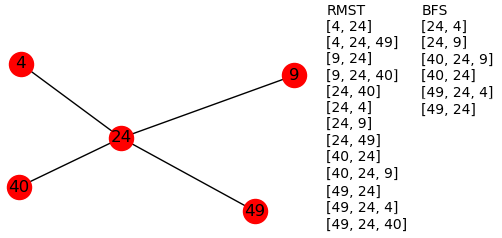
\includegraphics[scale=0.8]{imagenes/BFSvsRMSTpaths.png}
        \caption{Subconjunto {\bf P'} para el grafo de 5 nodos a la izquierda, utilizando la opci\'on de 100 {\it RMST} o heur\'istica de {\it BFS} que corta el camino al encontrar un \'angulo de deflexi\'on mayor a 60\degree entre aristas adyacentes.  }
        \label{fig:subconjunto-p-prima-caminos-posibles}
    \end{subfigure}
    \caption{(\ref{fig:define-set-cover}) A partir de un grafo ponderado proveniente de una estructura sint\'etica o de una imagen real, se elige {\bf P'} entre los $N(N-1)/2$ caminos no triviales y sin direcci\'on que aporta cada uno de los 100 \'arboles de expansi\'on m\'inima aleatoria ({\it RMST}), o los caminos resultantes de la heur\'istica de b\'usqueda por anchura ({\it BFS}) con interrupci\'on al dar con una arista que tenga un \'angulo superior a 60\degree. (\ref{fig:subconjunto-p-prima-caminos-posibles}) Subconjunto {\bf P'} de P, para el grafo de 5 nodos de ejemplo a la izquierda. }
    \end{figure*}
    
    
Este enfoque faculta que al tener un grafo que representa la red de filamentos, como en la figura \ref{Fig1d}, sea posible llegar a resultados como los que aparecen en las figuras \ref{Fig2a} o \ref{Fig2b} a trav\'es de la asignaci\'on de pesos a la aristas, y de restricciones a las uniones entre las mismas. Cabe destacar que el {\it FCP} s\'olo utiliza 2 caracter\'isticas independientes para describir los segmentos de los filamentos, siendo el \'angulo de deflexi\'on entre aristas usado en la etapa de selecci\'on de subconjuntos de caminos s\'olo si es seleccionada la heur\'istica {\it BFS}, y el grosor, empleado para describir el peso de las aristas.  
%es de complejidad $\mathcal{O}(N^{(2K+2)})$, con $N$ como n\'umero de nodos y $k$ como el n\'umero m\'aximo de caminos que pasan por cada v\'ertice. 
% Aquello permitir\'ia pasar de Fig1d a Fig2b por ejemplo

En ambas categor\'ias, las cr\'iticas m\'as repetidas en los trabajos del \'area suelen ser la cantidad de par\'ametros y la dificultad en su ajuste, en las diversas herramientas existentes. Un segundo problema com\'un es que la obtenci\'on de informaci\'on relacionada a la morfolog\'ia y el comportamiento de las redes es m\'as cualitativo que cuantitativo \cite{asgharzadeh2018computational}\cite{qiu2014quantitative}, lo que supone un problema al trasladar el  an\'alisis a una gran cantidad de datos, dado que cada enfoque es demasiado espec\'ifico a su correspondiente software.

\medskip

\begin{figure*}[h]
    \begin{subfigure}[t]{0.5\textwidth}
        \centering
        
\includegraphics[height=1.2in]{imagenes/define-weighted-4-expected2.png}
        \caption{Visualizaci\'on de un resultado posible de individualizaci\'on, limitando los filamentos identificados a estructuras simples.}
        \label{Fig2a}
    \end{subfigure}%
    ~ 
    \begin{subfigure}[t]{0.5\textwidth}
        \centering
        
\includegraphics[height=1.2in]{imagenes/define-weighted-4-expected1.png}
        \caption{Visualizaci\'on de otro resultado posible de individualizaci\'on, permitiendo filamentos m\'as complejos.}
        \label{Fig2b}
    \end{subfigure}
	\caption{Posibles resultados de la identificaci\'on de filamentos. El resultado esperado de esta investigaci\'on es asociar a cada arista del grafo, como el de la figura \ref{Fig1d}, un peso que pondere diversos criterios como \'angulo de bifurcaci\'on del filamento, grosor y/o largo. Al plantearlo como un problema de optimizaci\'on, la ponderaci\'on y otras restricciones, entregar\'an resultados como la imagen \ref{Fig2a} o \ref{Fig2b}, expresado gr\'aficamente mediante gradiente de colores. Fuente: Elaboraci\'on propia}
\end{figure*}


%\begin{teo}
%Se tiene que $$\int_0^t e^sds=e^t-1.$$
%\end{teo}
\end{intro}